
According to IDC (www.idc.com) -- a global provider of market intelligence, advisory services, and events for the information technology, telecommunications and consumer technology markets -- the worldwide shipment of smart connected devices will surpass 2.5 billion units in 2017. As the cost, size, and power requirements keep decreasing, computing will be embedded in all kinds of products and everything that can benefit from the Internet will be connected. Not only stations, computers or laptops, but also tablets, smartphones, cars, game consoles, TV sets, cameras, machines, lights, locks, and home appliances.\\

People and data are already online. Soon, all sort of things with sensors, actuators and places will be also online. All sectors of activity will benefit from applications that leverage the interconnection of embedded systems with IT systems. Intelligent transport solutions can speed up traffic flows, reduce fuel consumption, and safe lives. Smart farming solutions will improve the production and delivery of safe and healthy food. Remote health monitoring will provide convenient access to healthcare, raises it quality, and save money. Utilities management, education, government services, retail sectors etc.… all will also benefit from such couplings and the things will leave across all different systems. \textbf{The next step is to interconnect these individual systems into a system of systems, and here we are confronted to such a scale and heterogeneity that we are reaching a limit in networking and software engineering}.\\

In this project, we aim to investigate issues related to the design and development of a secure physical and computational networked environment, consisting of billions of connected smart objects (things), which allows interoperability and facilitates efficient collection and processing of data and analytics. These smart objects may come from diverse environments such as smart appliances at homes, smart mobile surveillance system such as fire trucks and police cars, smart transportation entities (e.g., cabs or buses), etc. By establishing a dynamic instantiations of Internet of Things (IoT) structures, we aim to  provide an automatic resource optimization and other intelligence into these evolving collections of smart connected objects. However, rather than endowing them with autonomously cognitive chips, we ask for manufacturers, retailers and users/owners, through an established social network of things, to elaborate finely tuned dispatches to be distributed toward the smart objects through middleware fogs located in the individual homes. \\

Nowadays, existing start of the art related to the design of IoT systems is highly compartmentalized, the data collection and analytics processing across a variety of heterogeneous IoTs has limited support, and the interoperability of objects across domains has not been addressed at a level that would provide the kinds of optimizations that this project aims.. In this project, we introduce the concept of collaborative Social Network of Things that would enable data and analytics sharing across objects that exhibit similar operating characteristics and/or have similar profiles in terms of usage and user/manufacturer parameters. In addition, we propose to develop a hierarchical middleware implemented as fogs to allow interoperability with context-aware security properties associated with different nodes. These middleware fogs, mainly implemented in smart boxes/gateways within local networks, will manage the communication between the associated smart objects and the network in an optimized way that takes into account both the characteristics of the smart objects and the preferences of the users. The massive generated data by all these connected smart objects and stored in the system will enable the cognitive network, through deep learning algorithms, to raise dynamic procedures that will enable a multi-criteria optimizations of the  behavior  of these smart objects.\\

A typical scenario could be as follows. During his  coffee break at the office, Jack decides to lower by 5 degrees the set point temperature of his home heating system – which must go into action when he is less than 1 mile from his home and in any case no later than 6PM. However, if the outside temperature drops below certain threshold, the temperature must go up by 5 degrees. At lunchtime, a colleague of his gives Jack a list of instructions corresponding to a new method for washing wool sweaters; he  sends the file directly to his home through the social network where a service will adapt the instructions to that washing machine’s particular technical features and his personal preferences for extra soft cloths. Back at home, Jack launches “my angry day” profile through  smartphone, which automatically dims the light and has the Hi-Fi play his favorite relaxing music. Meanwhile, a tip from the network tells Jack to turn off all TVs to avoid getting further depressed. During the night the washing machine starts the cycle at the time the electric company informs it to be the most favorable.\\

While the above describes a single user, what we aim to investigate in this project is how to incorporate multiple users and smart devices into multiple instances of Social Network of Things, that can be generated/organized and dissolved on-the-fly; where different criteria can be used to orchestrate the behavior of (groups of) instances subject to multiple constraints; and certain security and privacy concerns are ensured. In the context of “Jack” scenario, this would mean collaboratively regulating the temperature with other units in Jack’s building; collaboratively deciding about the cycle of the washing machine in terms of optimizing the grid-demand within a city-block; adjusting the Hi-Fi themes based on the fact that Jack decided to join his co-workers for a happy-hour; etc… Moreover, we plan to provide novel data analytics methodologies that will: (a) incorporate the fact that some users may not be cooperative in terms of suggested regime of use for certain devices/task; (b) provide a specific behavioral insights to be used by various manufacturers when planning the design of certain devices so that they can be better adapted to changing conditions of use. 
The architecture we target to support such  scenarios is depicted in Figure 1. We aim at providing methodologies and tools for two basic modes: \\

\begin{wrapfigure}{R}{0.30\textwidth} \vspace{-3mm}
	\centerline{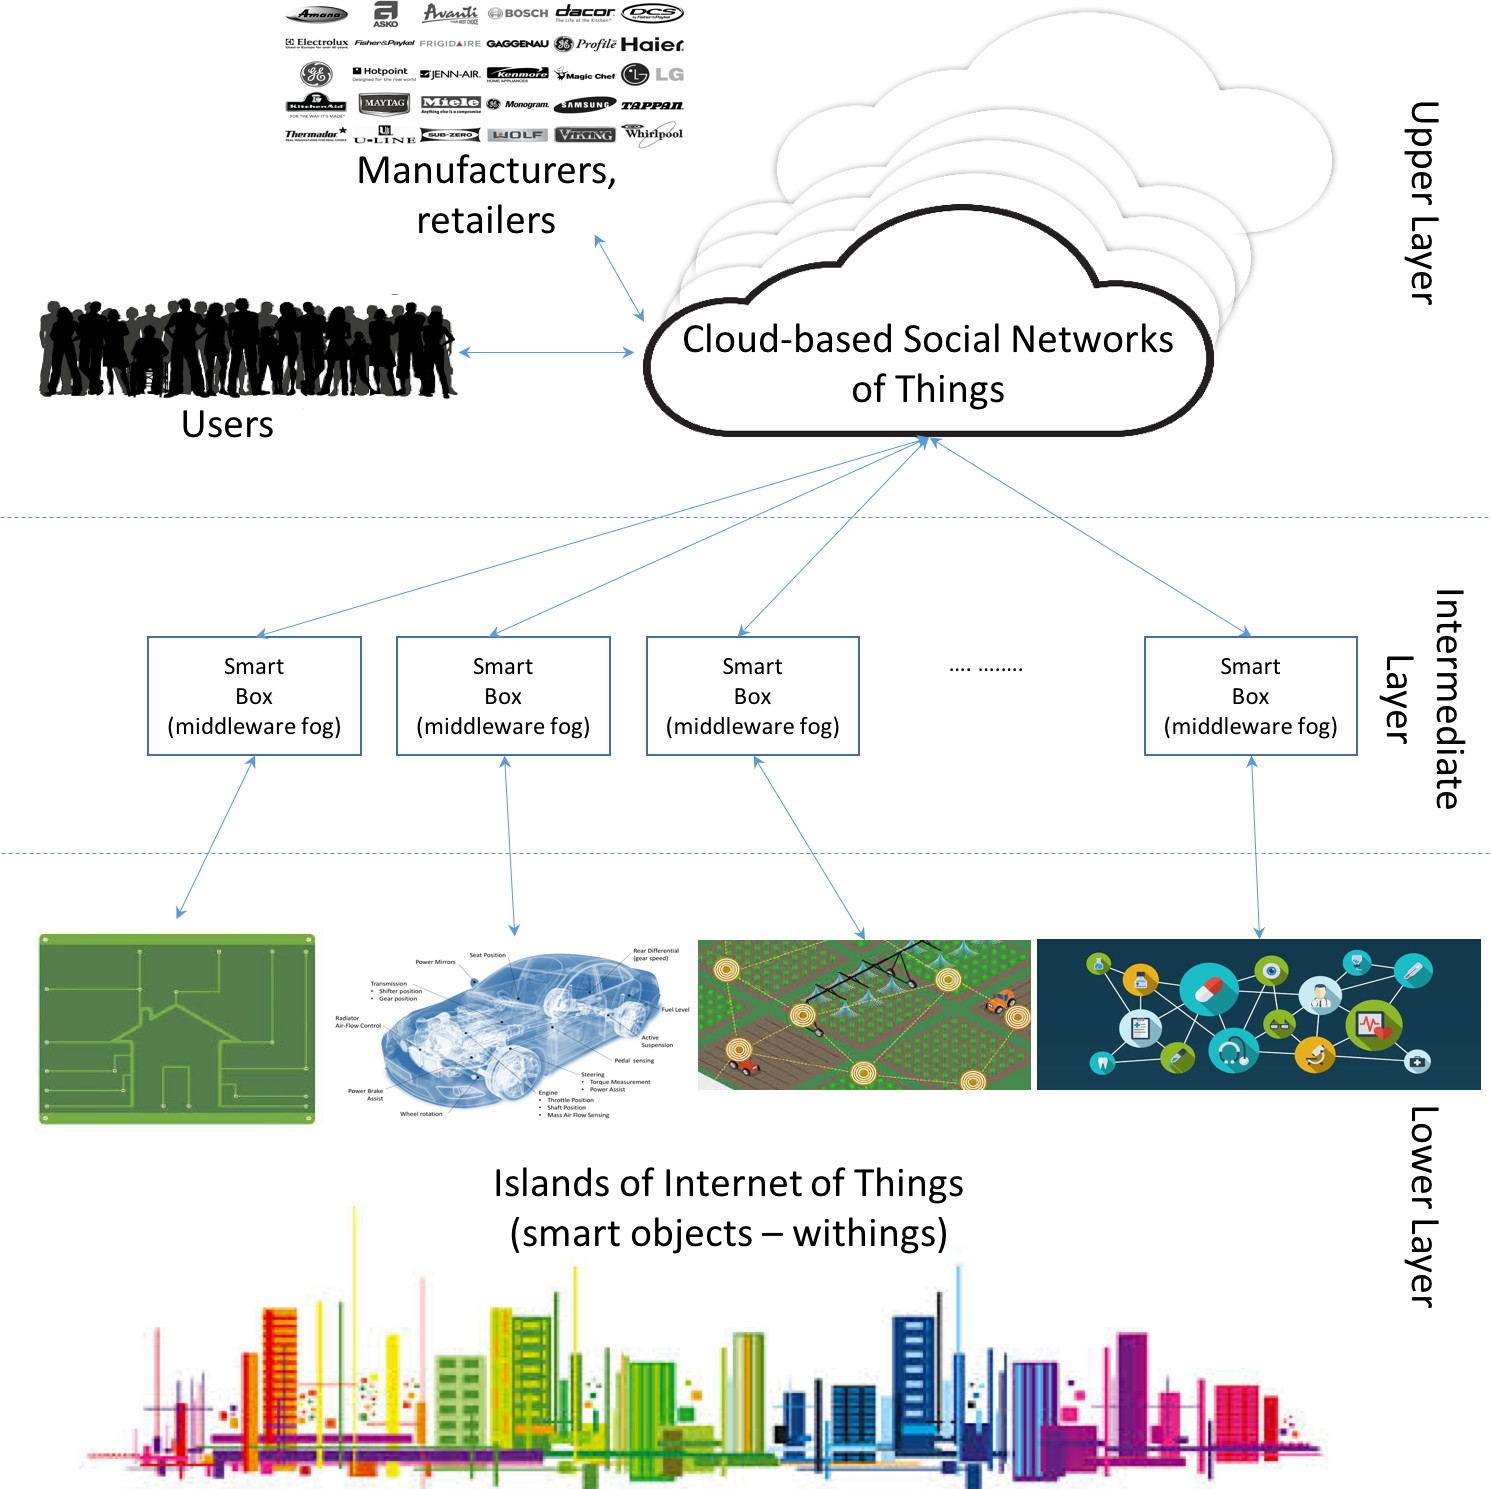
\includegraphics[width=0.30\textwidth]{./fig1.png}}
	\vspace{-3mm} \caption{\small An overview of the system}
	\label{fig1}
	\vspace{-3mm}
\end{wrapfigure}

(1)  The first setup consists of a set of middleware fogs, located in each smart box/gateway of a smart home or public area, grouped together in a social network along with profiles of manufacturers, retailers and users/owners. The lower layer is formed by all the real devices/objects (things), such as a fridge, a washing machine, a heater, a TV, a Hi-Fi, etc., where each one is abstracted by what we refer to as WiThing (WiT) for Wireless Thing. The WiT is the first level of the device abstraction and its role is to (1) uniquely identify an object/device worldwide, (2) represent the object in terms of its properties/functionalities through an MIB (Management Information Base), and (3) constitute a bidirectional interface for all communications between the object and the middleware fog located in the smart box/gateway. The intermediate layer contains the smart box/gateway where the middleware fog is implemented. The latter is composed of an ensemble of interconnected modules that will govern all the requests issued by the user through a proper front-end application. To this end, this smart box must interface with any object/device it meets in the surroundings, i.e., any virtual device communicated by the real objects/devices. The upper layer contains the social networks of manufacturers, retailers and users/owners with the generic representations (avatars) of their objects/devices. It consists of a large database with an enquiry system based on sophisticated algorithms.
Throughout this complex environment, and in order to fully automate the deployment and control of such Internet of Things, gathering of important data, identification of correlations in this chain of complex events, and triggering the required responses, a plethora of issues in data collection and processing (storage/retrieval, querying and information fusion), knowledge discovery, and security and privacy need to be investigated in unified framework. We assert that  such integrated large scale effort, involving researchers from diverse backgrounds, is necessary to  enable exploiting the full potential of the Internet of Things technology  and make it ubiquitous of use.\\

(2) The second setup complements the previous one in terms of inter-contexts couplings and dynamic formations (and dissolution) of corresponding Avatars. In terms of notation in Figure 1. it is best explained by the following scenarios:
(a) If we have a collection of Avatars corresponding to a particular device (e.g., a washer) in a collection of residential units, depending on the geographical context we may want to form different instances of (meta)Avatars corresponding a group of same devices but operating in: (i) a group of houses in a suburban residential area; and/or (ii) a group of buildings in a near-downtown area.
(b) Complementary to this, the Avatars corresponding to washers in different units in an apartment complex, may be tied with the Avatars corresponding to entertainment devices in the same and/or neighboring buildings.
(c) The collection of Avatars representing the traffic-density in different geographical regions may be tied with the crime-rate in those and/or near-by regions and with the ones corresponding to activities of electronic devices in the police cars. However, after a certain time of the day/night, such (meta)Avatars may cease to exist. 

The situational awareness that we aim to capture by dynamically creating Meta-Avatars is illustrated in Figure 2. We note that, in addition to the scenario-oriented discussion above, the Meta-Avatars may be created based on:\\

\begin{wrapfigure}{R}{0.30\textwidth} \vspace{-3mm}
	\centerline{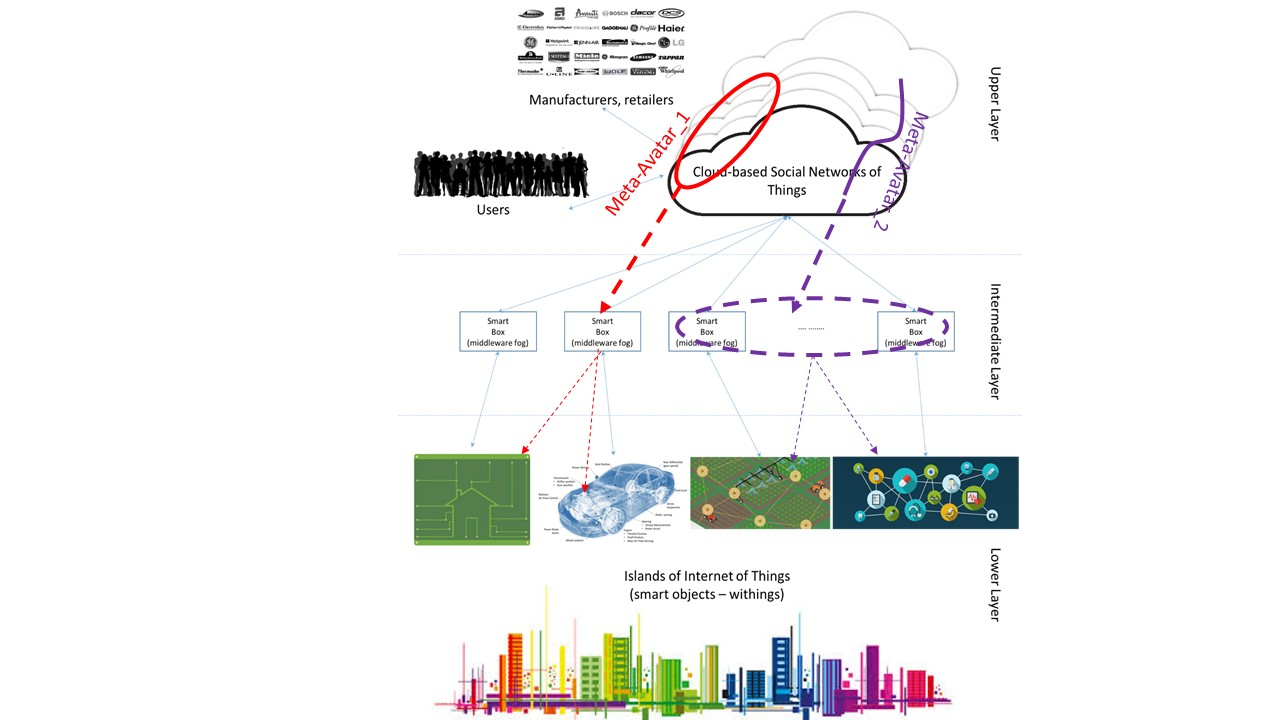
\includegraphics[width=0.30\textwidth]{./fig2.jpg}}
	\vspace{-3mm} \caption{\small Meta-avatars}
	\label{fig1}
	\vspace{-3mm}
\end{wrapfigure}

-	Particular cyber-properties: e.g., status of network infrastructure, privacy constraints, etc.
Logical or semantical properties which may entail dynamically forming (and dissolving) hierarchies of such avatars.\\

The main Intellectual Merits of the proposed project are:
----Repeat the Intellectual Merits here…
